\documentclass[tikz,border=0pt]{standalone}
\usepackage[american]{circuitikz}
\usetikzlibrary{arrows.meta,calc,positioning,decorations.pathmorphing,patterns}
\definecolor{zyloTeal}{HTML}{174A5B}
\definecolor{zyloTealTwo}{HTML}{246B7A}
\definecolor{zyloInk}{HTML}{1F2933}
\definecolor{zyloSoft}{HTML}{EAF4F4}
\definecolor{zyloPaper}{HTML}{F8FAFB}
\definecolor{zyloLine}{HTML}{44606B}
\definecolor{zyloOrange}{HTML}{D97706}
\begin{document}
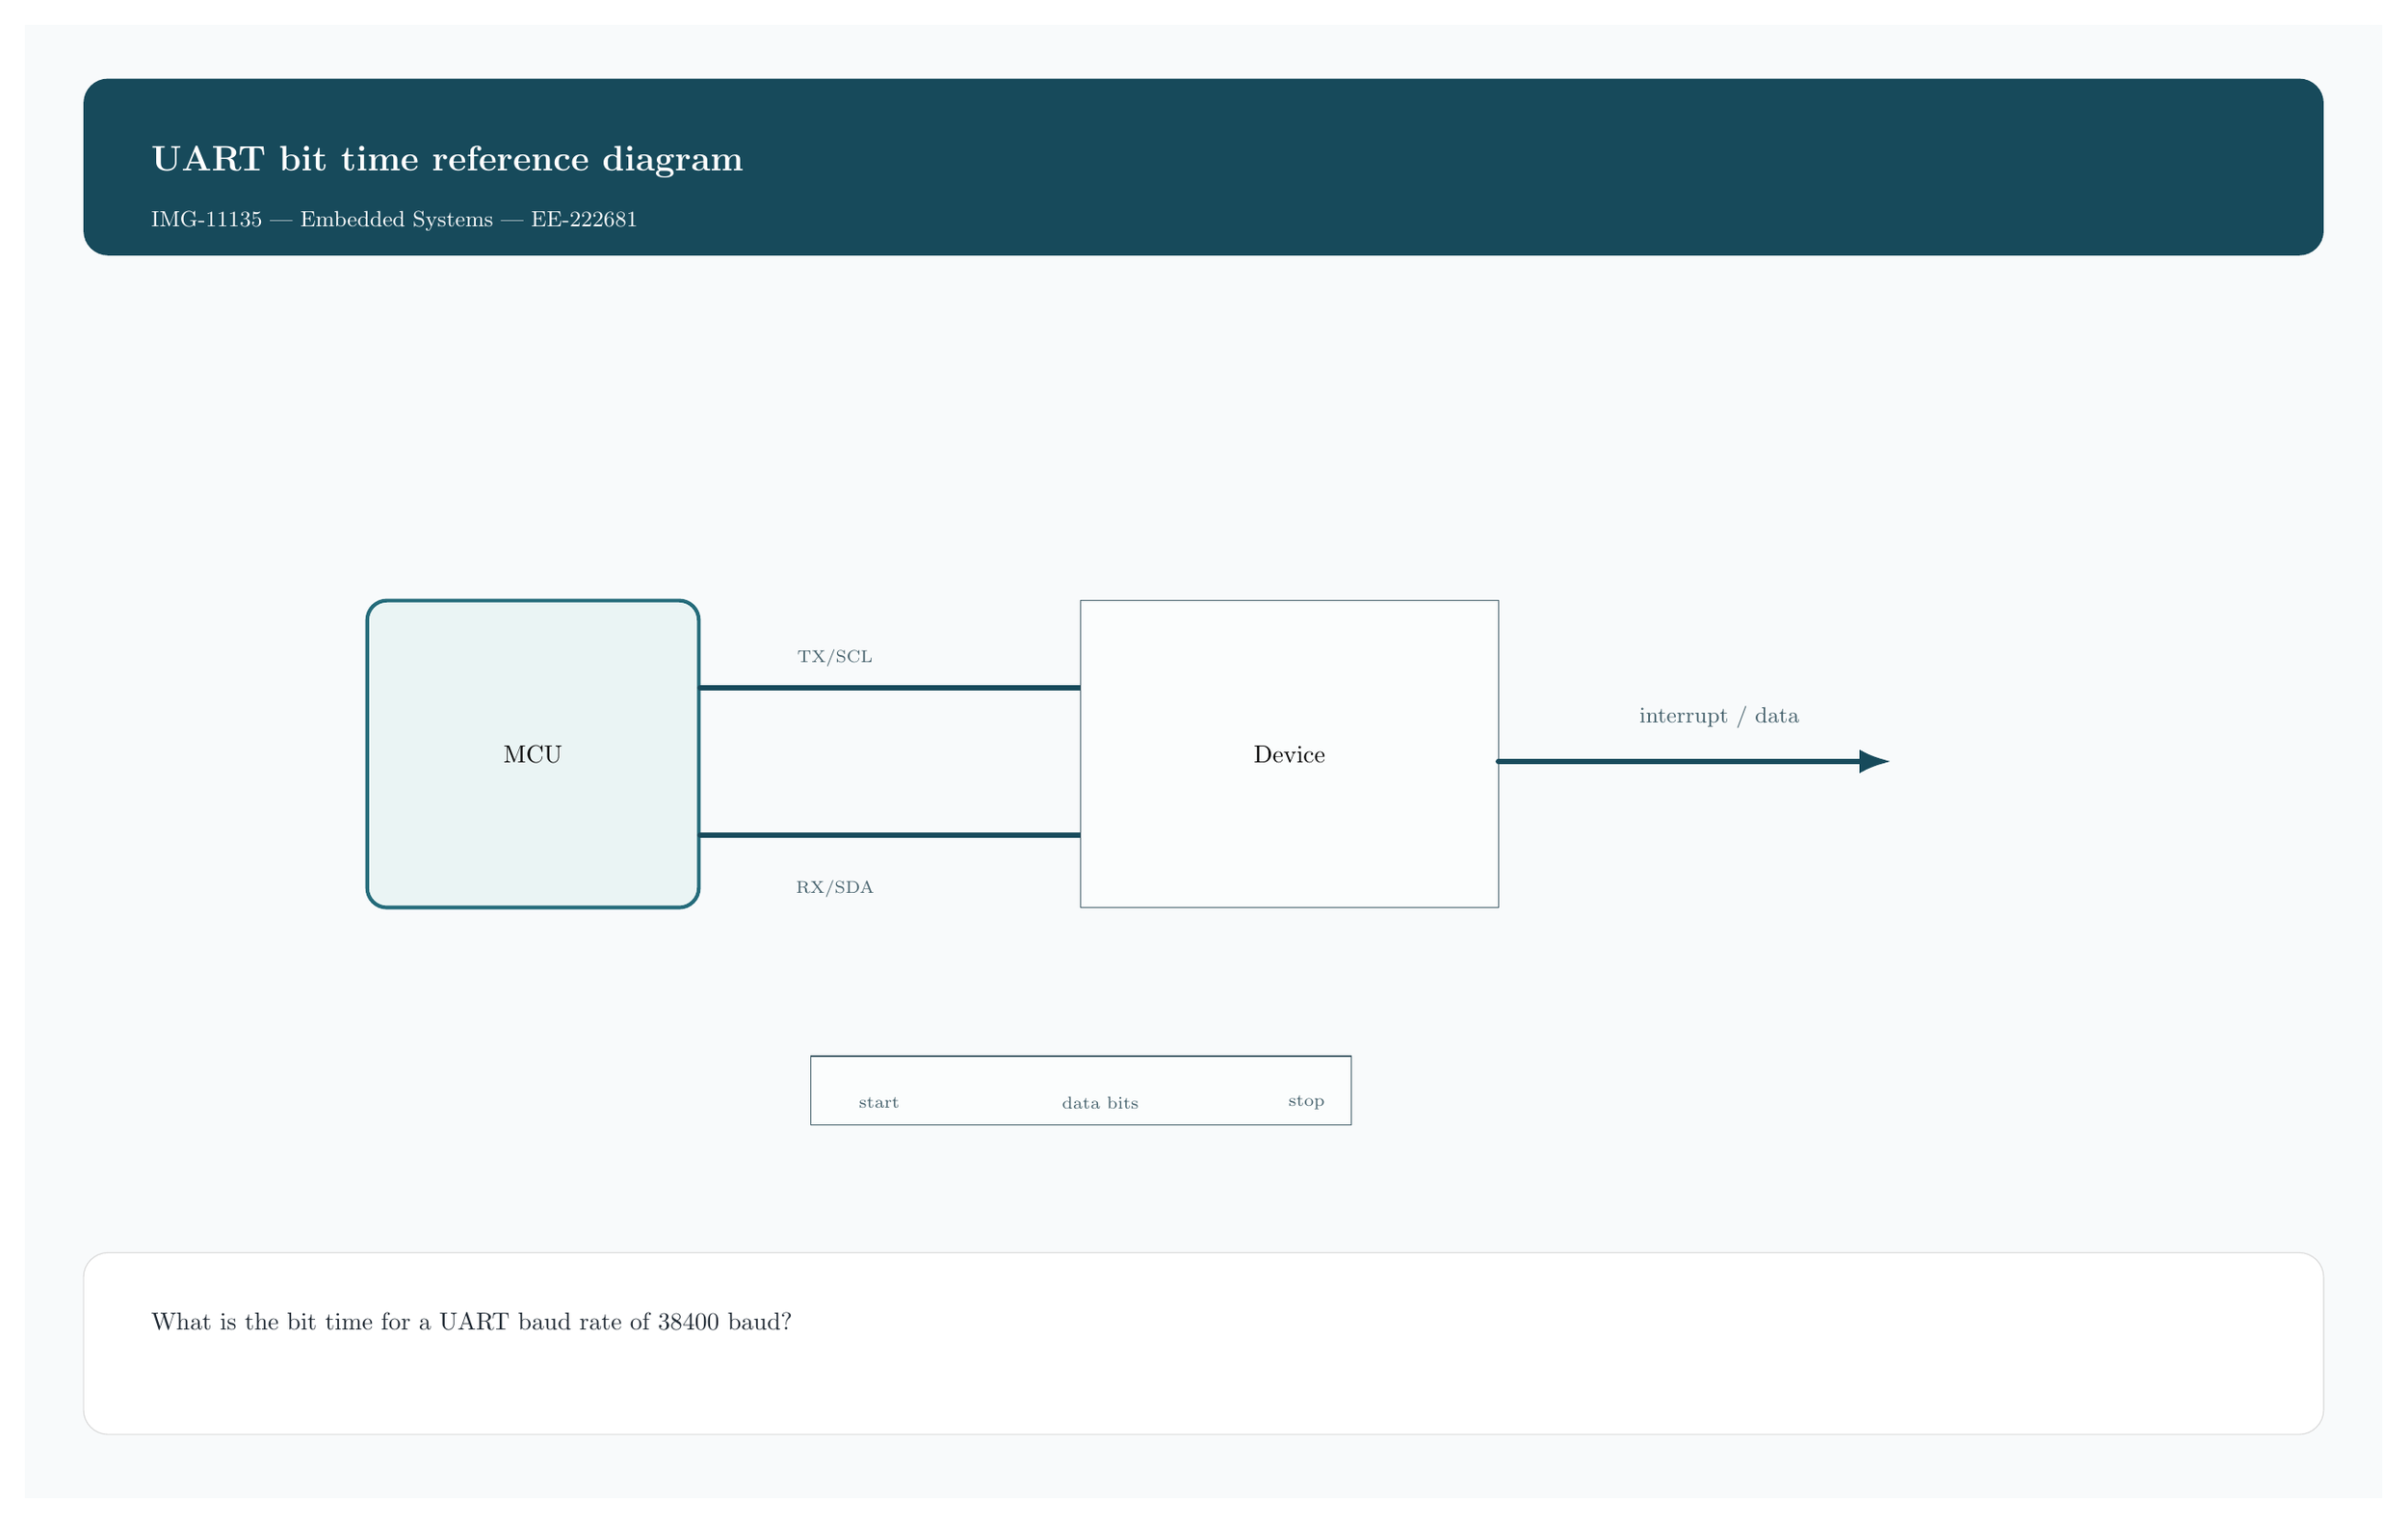
\begin{tikzpicture}[x=1pt,y=-1pt,>=Latex,line cap=round,line join=round]
\path[fill=zyloPaper] (0,0) rectangle (960,600);
\path[fill=zyloTeal,rounded corners=10pt] (24,22) rectangle (936,94);
\node[anchor=west,text=white,font=\bfseries\Large] at (48,56) {UART bit time reference diagram};
\node[anchor=west,text=white!82,font=\small] at (48,80) {IMG-11135 | Embedded Systems | EE-222681};
\tikzset{wire/.style={draw=zyloTeal,line width=2.2pt},thinwire/.style={draw=zyloLine,line width=1.35pt},accent/.style={draw=zyloOrange,line width=2.2pt},box/.style={draw=zyloTealTwo,fill=zyloSoft,line width=1.5pt,rounded corners=8pt}}
\node[box,minimum width=135pt,minimum height=125pt] at (207,297) {MCU};
\draw[wire] (275,270) -- (430,270); \draw[wire] (275,330) -- (430,330);
\node[font=\scriptsize,text=zyloLine] at (330,258) {TX/SCL}; \node[font=\scriptsize,text=zyloLine] at (330,352) {RX/SDA};
\node[draw=zyloLine,fill=white!80!zyloSoft,minimum width=170pt,minimum height=125pt] at (515,297) {Device};
\draw[wire,->] (600,300) -- (760,300); \node[font=\small,text=zyloLine] at (690,282) {interrupt / data};
\path[draw=zyloLine,fill=white!80!zyloSoft] (320,420) rectangle (540,448);
\node[font=\scriptsize,text=zyloLine] at (348,439) {start}; \node[font=\scriptsize,text=zyloLine] at (438,439) {data bits}; \node[font=\scriptsize,text=zyloLine] at (522,439) {stop};
\path[draw=black!15,fill=white,rounded corners=10pt] (24,500) rectangle (936,574);
\node[anchor=west,text width=860pt,align=left,text=zyloInk,font=\normalsize] at (48,528) {What is the bit time for a UART baud rate of 38400 baud?};
\end{tikzpicture}
\end{document}
